\begin{figure}[!p]
\centering
\resizebox{\linewidth}{!}{\sffamily
{(a)} \begin{tabular}{c|c|c|c|c|c|c}
\texttt{\#86} (355 nt) & Boltzmann prob. & ensemble defect & struct. distance & energy gap & & \\
``Methaqualone'' & $p(\vecystar \mid \vecx)$$(\uparrow)$ & \NED$(\vecx, \vecystar)$$(\downarrow)$ & $d(\MFE(\vecx), \vecystar)$$(\downarrow)$ & \DDG$(\vecx, \vecystar)$$(\downarrow)$ & is \MFE & is uMFE \\
\hline
EliteDesign ($N=500$) & {\boldmath$4.28 \times 10^{-6}$} & \textbf{0.066} & \textbf{12} & \textbf{6.1 kcal/mol} & No & No \\
SamplingDesign & $3.87 \times 10^{-7}$ & 0.112 & \textbf{12} & 6.5 kcal/mol & No & No \\
\hline
Probability ceiling & $6.95 \times 10^{-5}$ & --- & --- & --- & --- & --- \\
\end{tabular}}\\[5pt]
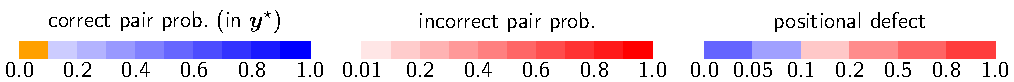
\includegraphics[width=0.9\linewidth]{figures/structures/legend}\\[3pt]
{\sffamily\small
\begin{tabular}{@{}c@{\hspace{0.01\linewidth}}c@{\hspace{0.01\linewidth}}c@{}}
(b) Target \vecystar & (c) \MFE structure of EliteDesign ($N=500$) & (d) \MFE structure of SamplingDesign \\[2pt]
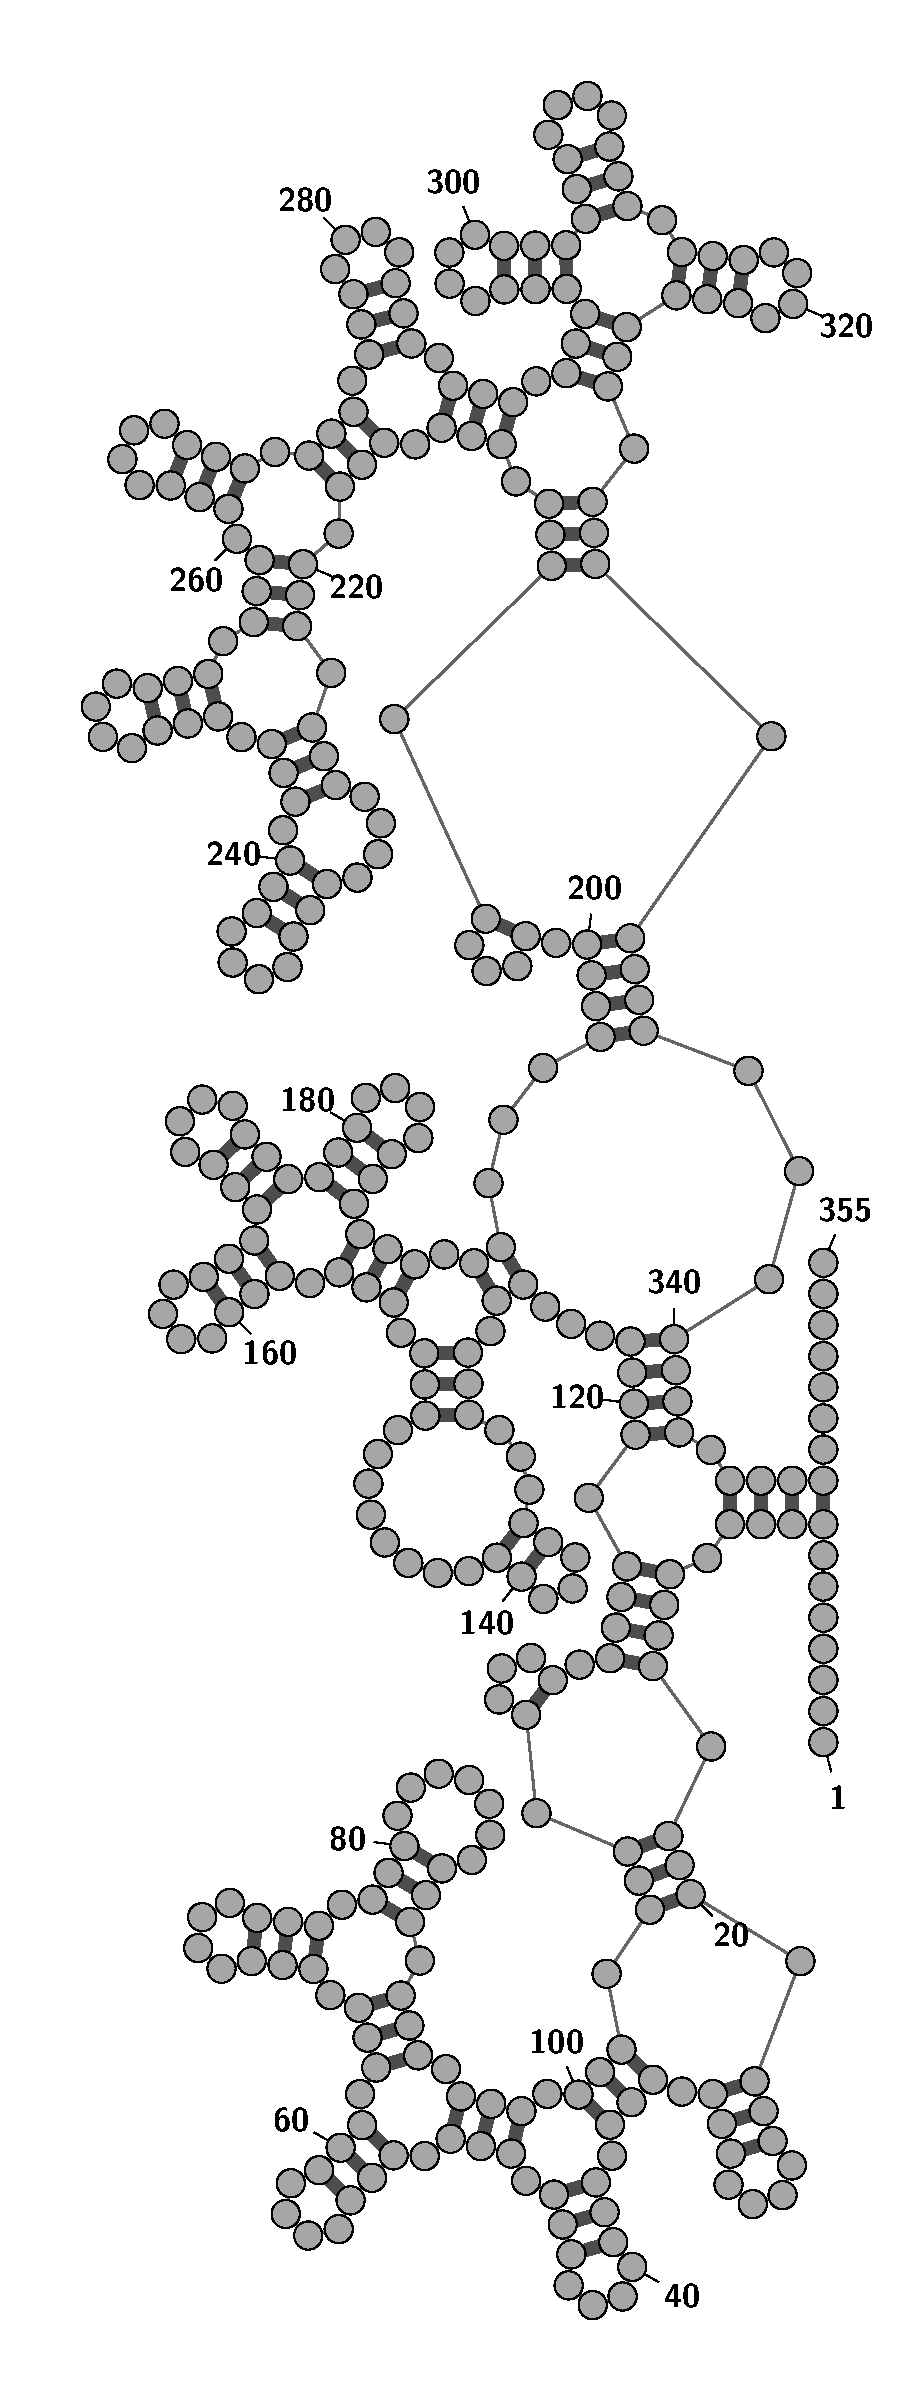
\includegraphics[height=4.9in]{figures/structures/target_86} &
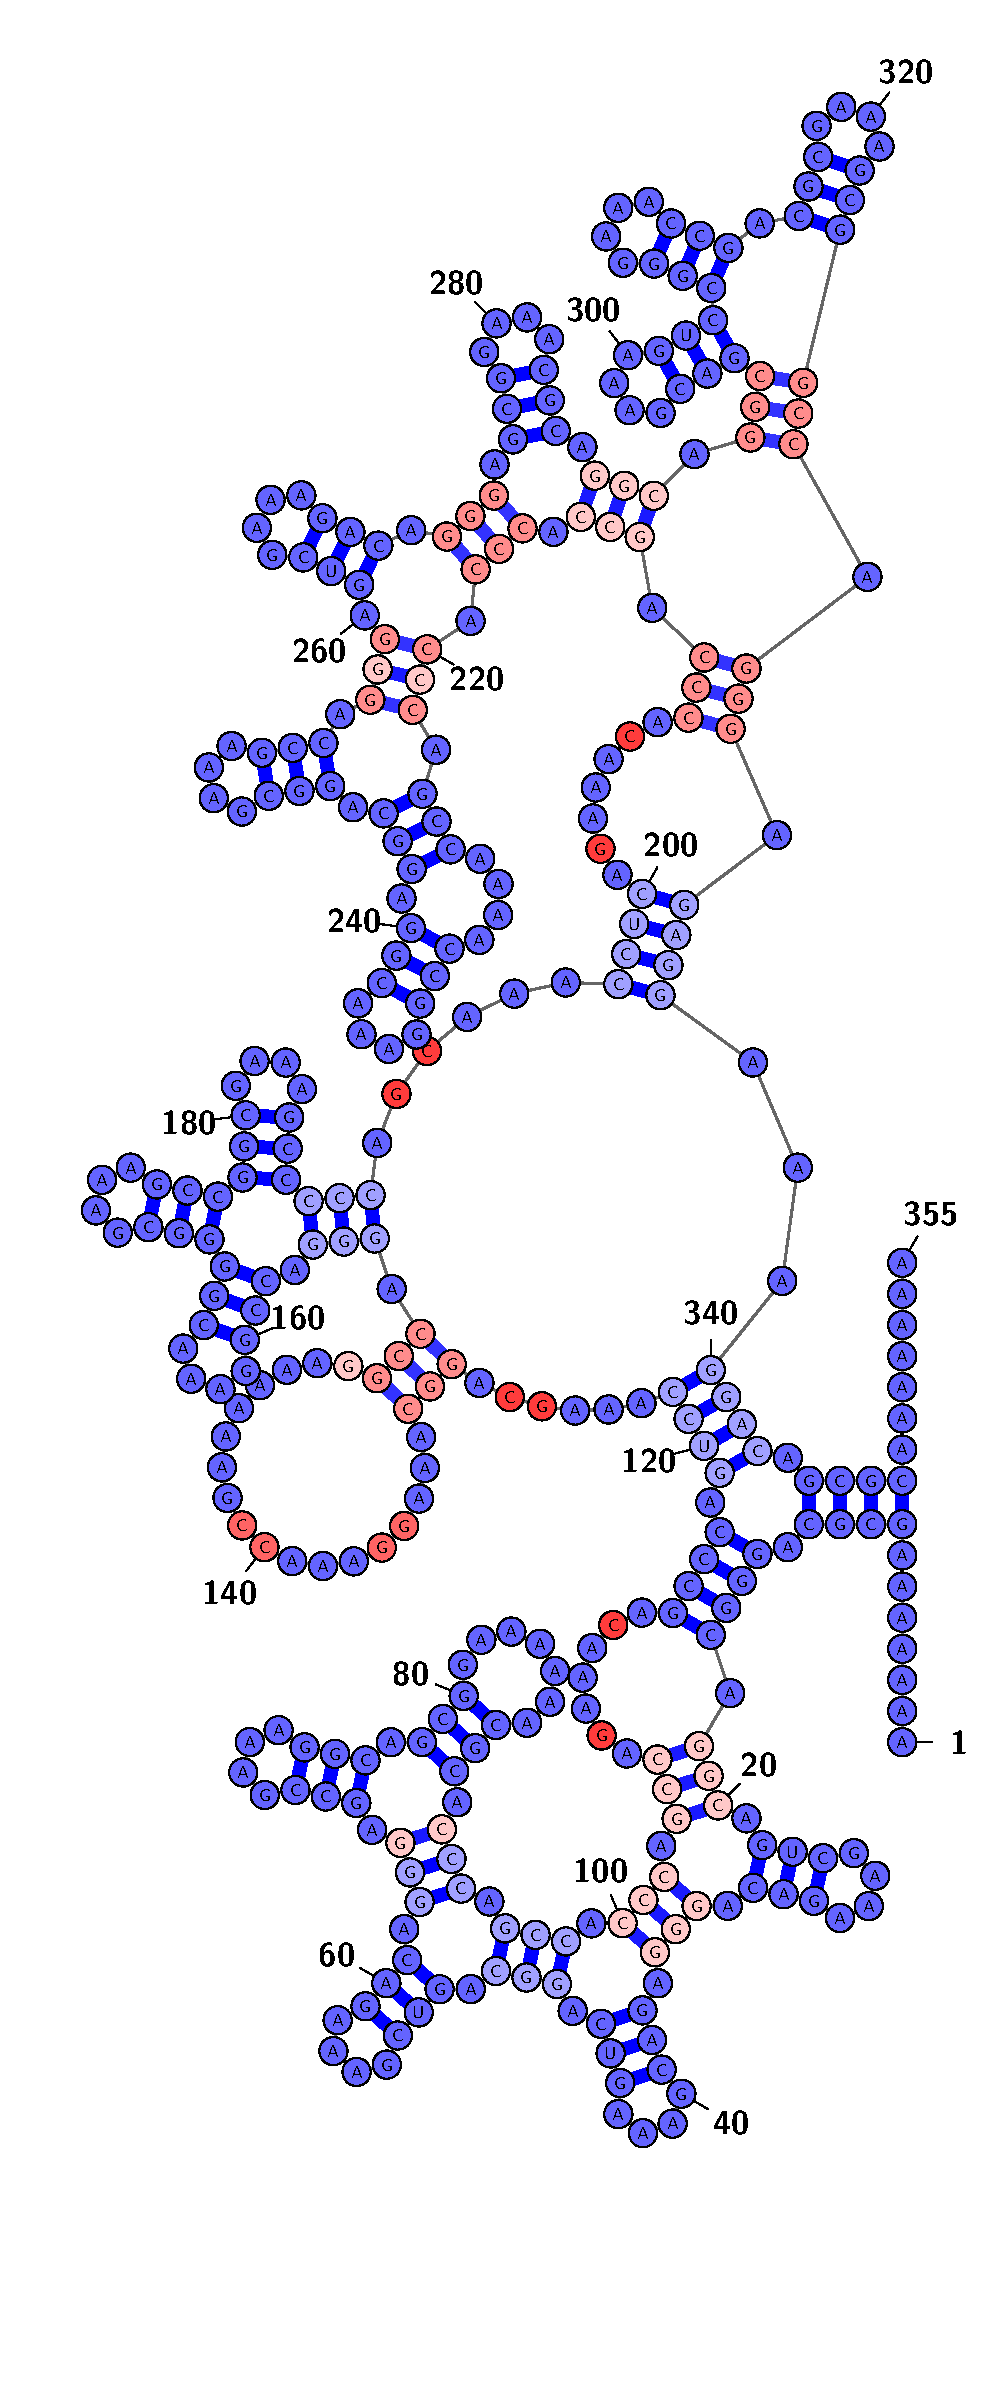
\includegraphics[height=4.9in]{figures/structures/structure_86_elite} &
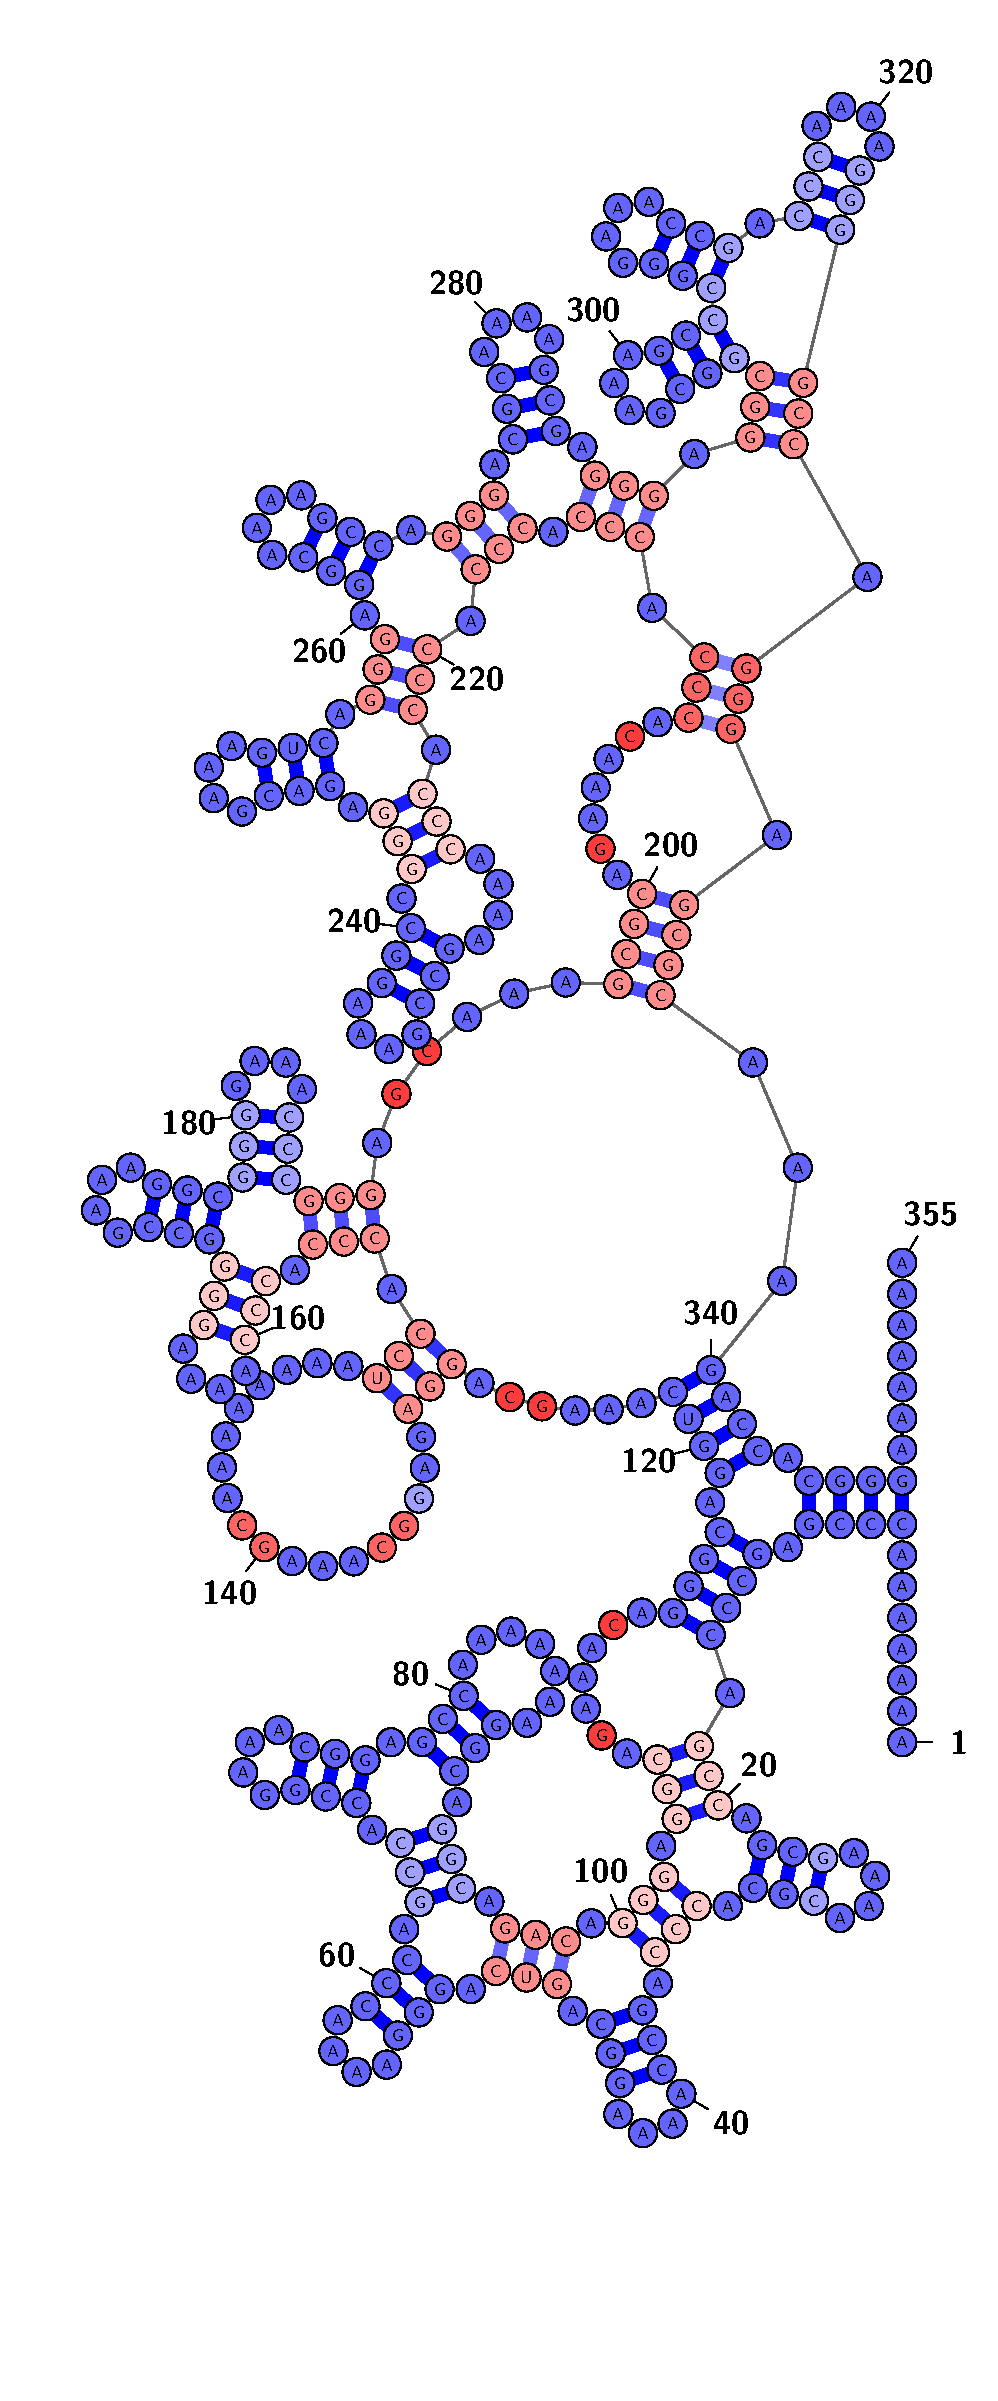
\includegraphics[height=4.9in]{figures/structures/structure_86_sampling}
\end{tabular}\\[3pt]
\begin{tabular}{@{}c@{\hspace{0.02\linewidth}}c@{}}
(e) Base-pairing probabilities, EliteDesign ($N=500$) & (f) Base-pairing probabilities, SamplingDesign \\[1pt]
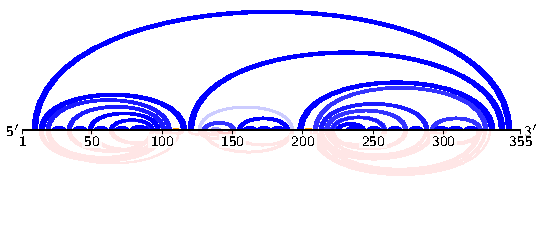
\includegraphics[width=0.49\linewidth]{figures/structures/arcs_86_elite} &
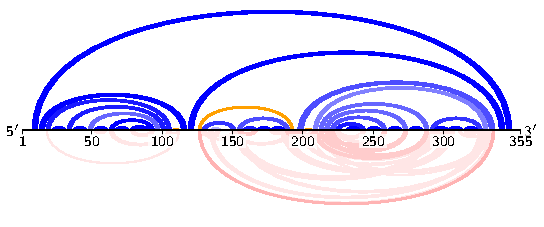
\includegraphics[width=0.49\linewidth]{figures/structures/arcs_86_sampling}
\end{tabular}}
\caption{}
\label{fig:eterna-structure-86}
\end{figure}
